\section{Car Rental}

\subsection{Software Architecture and Methodologies}

\begin{frame}{Car Rental}
    \begin{block}{Applicazione}
        Applicazione a microservizi sviluppata in \textit{Quarkus in Action}.
    \end{block}
    \begin{block}{Architettura}
        Composta da cinque microservizi:
        \begin{itemize}
            \item Billing-service
            \item Inventory-service
            \item Rental-service
            \item Reservation-service
            \item Users-service
        \end{itemize}
    \end{block}
\end{frame}

\begin{frame}{Car Rental}
    \begin{block}{Dipendenze}
        I microservizi principali hanno delle dipendenze esterne:
        \begin{itemize}
            \item Billing-service: MongoDB, Kafka, RabbitMQ.
            \item Inventory-service: MySQL.
            \item Rental-service: MongoDB, Kafka.
            \item Reservation-service: PostgreSQL, RabbitMQ.
        \end{itemize}
    \end{block}
\end{frame}

\begin{frame}{Car Rental}
    \begin{columns}
        \begin{column}{.45\textwidth}
            \begin{block}{Comunicazione}
                La comunicazione tra servizi avviene in vari modi:
                \begin{itemize}
                    \item REST
                    \item GraphQL
                    \item Kafka
                    \item RabbitMQ
                    \item gRPC
                \end{itemize}
            \end{block}
            \end{column}
            \begin{column}{.55\textwidth}
                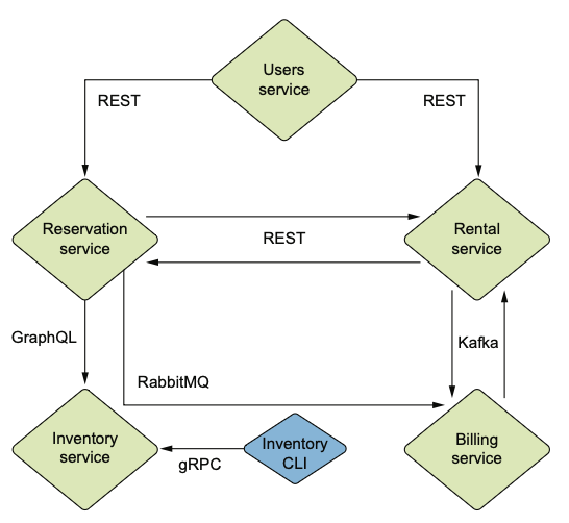
\includegraphics[width=\textwidth]{images/1-car rental/comunication.pdf}
            \end{column}
        \end{columns}
\end{frame}